\documentclass[10pt,tgadventor, onlymath]{beamer}

\usepackage{graphicx,amsmath,amssymb,tikz,psfrag,neuralnetwork, stackengine,array, multirow, fontawesome}

\input defs.tex
\graphicspath{ {./figures/} }

%% formatting

\mode<presentation>
{
\usetheme{default}
\usecolortheme{seahorse}
}
\setbeamertemplate{navigation symbols}{}
\usecolortheme[rgb={0.03,0.28,0.59}]{structure}
\setbeamertemplate{itemize subitem}{--}
\setbeamertemplate{frametitle} {
	\begin{center}
	  {\large\bf \insertframetitle}
	\end{center}
}


\AtBeginSection[] 
{ 
	\begin{frame}<beamer> 
		\tableofcontents[currentsection,currentsubsection] 
	\end{frame} 
} 


\usetikzlibrary{shapes,arrows}
\usetikzlibrary{positioning}
\tikzstyle{block} = [rectangle, draw, fill=blue!20, 
    text width=5em, text centered, rounded corners, minimum height=4em]
\tikzstyle{line} = [draw, -latex']



%% begin presentation

\title{\large \bfseries Power Allocation in Heterogeneous Networks for Base Stations with Multiple Antennas}

\author{Peter Hartig\\[3ex]
}

\date{\today}

\begin{document}

\frame{
\thispagestyle{empty}
\titlepage
}

\section{System Description}
\begin{frame}
\frametitle{The Heterogeneous Network}
	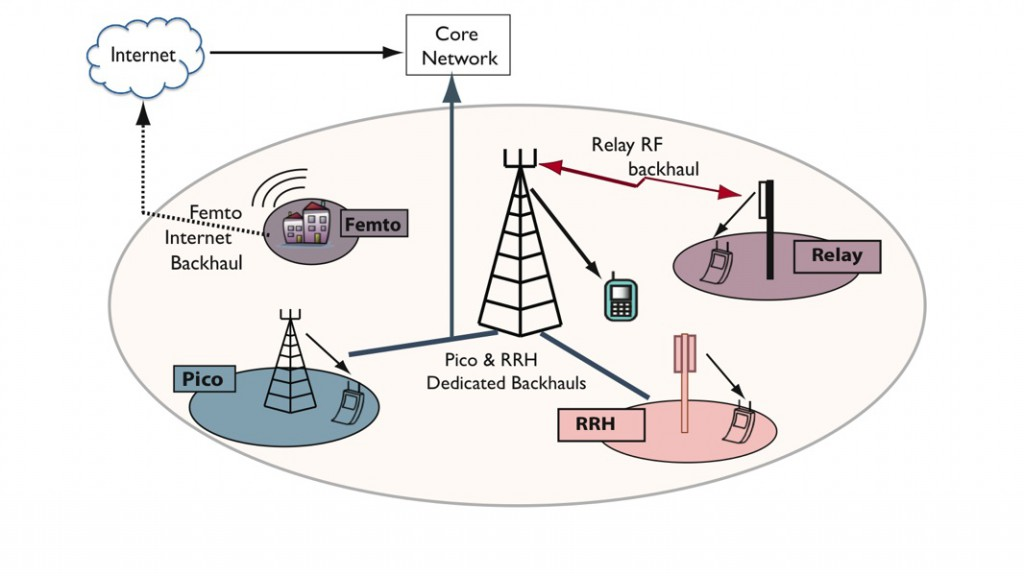
\includegraphics[width=\textwidth]{het_net}
\end{frame}


\begin{frame}
\frametitle{The Heterogeneous Network Game}
\begin{columns}

\begin{column}{0.5\linewidth}
	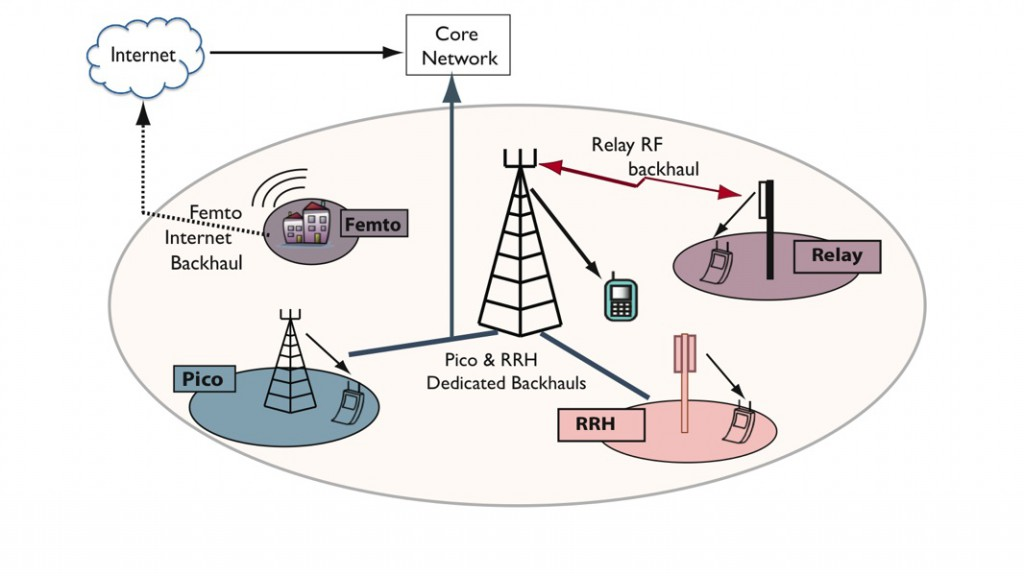
\includegraphics[width=\textwidth]{het_net}

\end{column}
\begin{column}{0.5\linewidth}
\begin{table}
    \setlength{\extrarowheight}{2pt}
    \begin{tabular}{cc|c|c|}
      & \multicolumn{1}{c}{} & \multicolumn{2}{c}{Player $2$}\\
      & \multicolumn{1}{c}{} & \multicolumn{1}{c}{$A$}  & \multicolumn{1}{c}{$B$} \\\cline{3-4}
      \multirow{2}*{Player $1$}  & $A$ & $(8,8)$ & $(2,15)$ \\\cline{3-4}
      & $B$ & $(15,2)$ & $(3,3)$ \\\cline{3-4}
    \end{tabular}
  \end{table}
\end{column}
\end{columns}
\bigskip
\begin{itemize}
\item 
	Players $=$ Femto Cell Base Stations (FCBS)
\item 
	Player Strategy $=$ FCBS Transmission Scheme
\end{itemize}

\end{frame}

%\begin{frame}
%\frametitle{The Heterogeneous Network Game}
%\begin{table}
%    \setlength{\extrarowheight}{2pt}
%    \begin{tabular}{cc|c|c|}
%      & \multicolumn{1}{c}{} & \multicolumn{2}{c}{Player $2$}\\
%      & \multicolumn{1}{c}{} & \multicolumn{1}{c}{$A$}  & \multicolumn{1}{c}{$B$} \\\cline{3-4}
%      \multirow{2}*{Player $1$}  & $A$ & $(8,8)$ & $(2,15)$ \\\cline{3-4}
%      & $B$ & $(15,2)$ & $(3,3)$ \\\cline{3-4}
%    \end{tabular}
%  \end{table}
%\bigskip
%\begin{itemize}
%\item 
%	Players $=$ Femto Cell Base Stations (FCBS)
%\item 
%	Player Strategy $=$ FCBS Transmission Scheme
%\end{itemize}
%
%\end{frame}


\section{Project Goals}

\begin{frame}
\frametitle{Objectives}
\begin{enumerate}
\setlength\itemsep{2em}

\item Find a Nash Equilibrium between all players.
\begin{itemize}
\item Preferably close to a social optimal.
\end{itemize}
\item Minimize resources required to reach Nash Equilibrium.
\end{enumerate}
%\pause
\begin{center}
%\begin{tikzpicture}{center}
%\node [block] (game) {Game with Many Players};
%\node [block, right = of game] (central) {Central Problem};
%\node [block, right = of central] (distributed) {Distributed Solution to Central Problem};
%
%\path[line] (game) -- (central);
%\path[line] (central) -- (distributed);
%
%\end{tikzpicture}
		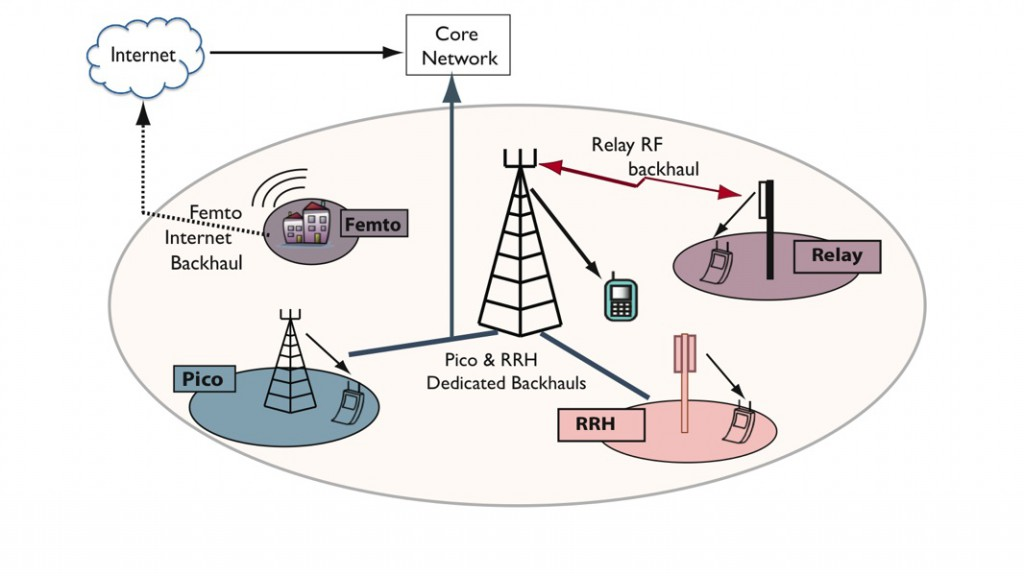
\includegraphics[scale=.2]{het_net}

\end{center}

\end{frame}

\section{Key Tools}

\begin{frame}
\frametitle{Key Tools: The Normalized Nash Equilibrium}
A Nash equilibrium in which the dual variables (prices) corresponding to constraints are equal up to a constant.
\begin{equation}
\lambda_f = \frac{\lambda_{0}}{ r_f}, \; \forall \; [r_0 \cdots r_F] > 0 
\end{equation}
Choosing $r_f =1$, all players must pay the same "price" to change their strategy. 
\end{frame}


\begin{frame}
\frametitle{Key Tools: N-Person Concave Games}
Conditions
\begin{itemize}
\item All Player utility functions must be concave with respect to their own strategy.
\item The set of strategies for the \emph{entire} game is convex. 
\end{itemize}
\bigskip
Implications
\begin{itemize}
\item Immediately proves existence of a \emph{pure strategy} Nash Equilibrium.
\item Provides an additional sufficient condition for uniqueness of Nash Equilibrium (diagonally strict concavity).
\end{itemize}
\end{frame}


\begin{frame}
\frametitle{Key Tools: Potential Games}
\begin{enumerate}
\item 
Potential Games
\begin{itemize}
\item "Central" optimization function $\Psi(\mathbf{s})$ with
\end{itemize}
\begin{equation}\label{potential_game_condition}
\frac{\partial \Psi(\mathbf{s})}{\partial \mathbf{s}_{f}}
 =
 \frac{\partial U_f(\mathbf{s})}{\partial \mathbf{s}_{f}}.
\end{equation} 
\item 
When all utility functions are strictly concave, the optimum of the potential function over the feasible set corresponds to a NNE.
\end{enumerate}
\end{frame}

\begin{frame}
\frametitle{Key Tools: Distributed Optimization}
Some optimization problems may be decomposed into "sub-problems".
\begin{equation}
f(x) = \sum_{i = 1}^{F} f_{i}(x_{i})
\end{equation}
Decomposing the corresponding Lagrangian gives
\begin{equation}
L(x,y) = \sum_{i = 1}^{F} L_i(x_i,y)
\end{equation}
\end{frame}
%

\section{System Model}
\begin{frame}
\frametitle{System Model: Femto Base Stations}
Each FCBS is a player in the game and is characterized by:
\\
\begin{itemize}
\setlength\itemsep{2em}

\item 
	$T_{f}$ antennas to transmit to $K_{f}$ femtocell users ($T_{f} \geq K_{f}$).
\item 
	The transmitted 		
	signal is $\mathbf{s}_{f
	}= \mathbf{U}_{f}\mathbf{x}_{f}$ with $E[\mathbf{x}_{f}\mathbf{x}_{f}^H] = \mathbf{I}$.
\item 
	An average power constraint $E\{trace(\mathbf{U}_{f}^H\mathbf{U}_{f})\} \leq P^{Total}_{f} $.
\item 
	A utility function $U_{f}(\boldsymbol{\gamma}_{f}) =
	\sum_{i=1}^{K_{f}}
    	 U_{f,i}(\gamma_{f,i}) $
    	in which $U_{f,i}(\cdot)$ is a non-decreasing function.
\end{itemize}
\end{frame}

%\begin{frame}
%\frametitle{System Model: FCBS Users}
%User $i$ of FBS $f$ has signal to interference plus noise ratio (SINR)
%	\begin{equation*}
%	\gamma_{f,i} = \frac{\|\mathbf{h}^H_{f,i}\mathbf{u}_{f,i}\|^2}
%	{\sigma^2_{\text{noise}}   +
%	\underbrace{
%	 \sum_{\tilde{f}=1, \tilde{f}\neq f}^{f} \sum_{u=1}^{K_{\tilde{f}}}
%	\|\mathbf{h}^H_{\tilde{f},u}\mathbf{u}_{\tilde{f},i}\|^2}_{\mathrm{inter-cell}}
%	 + 
%	 \underbrace{
%	 \sum_{\tilde{k}=1, \tilde{k}\neq i}^{K_f}
%	 \|\mathbf{h}^H_{f,\tilde{k}}\mathbf{u}_{f,\tilde{k}}\|^2}_{\mathrm{intra-cell}}},
%	  \; i \in \{1 ... K_f\}
%	  \end{equation*}
%\end{frame}

\begin{frame}
\frametitle{System Model: Macro Users}
	Received interference constraint given by 
	\begin{equation}
	E\{\sum^F_{f=1} \mathbf{\tilde{h}}_{m,f}^T  \mathbf{U}_{f}					
	\mathbf{U}_{f}^{H} \mathbf{\tilde{h}}_{m,f}^*\} \leq I^{Threshold}		
	_{m}
	\end{equation}
	\bigskip
	\centering
		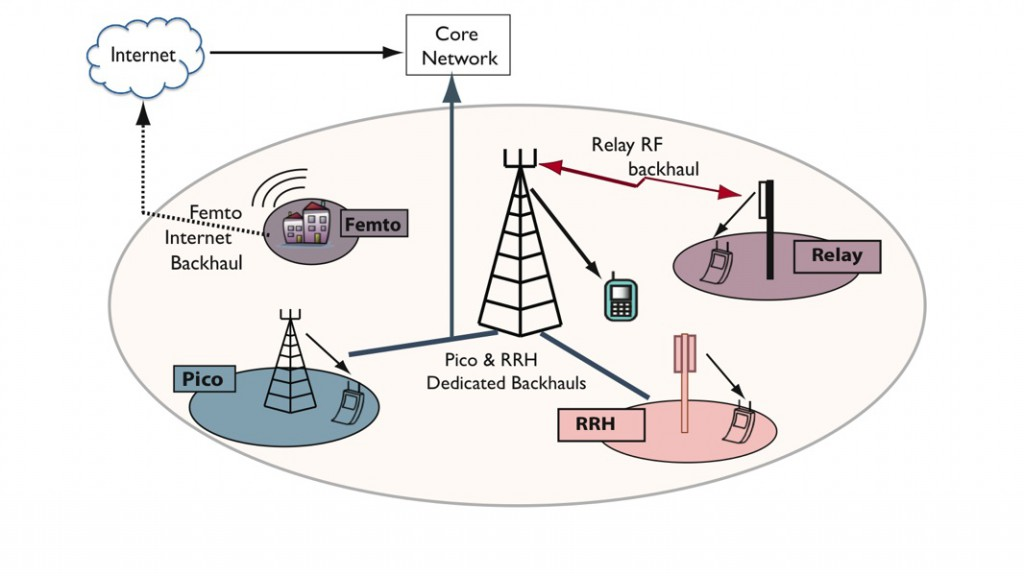
\includegraphics[scale=.2]{het_net}
\end{frame}

\begin{frame}
\frametitle{System Model: General}
\begin{itemize}
\setlength\itemsep{2em}

\item 
	No inter-femto cell interference
\item 
	FCBS have knowledge of channel state information 
	\begin{itemize}
	\item 
	The downlink channel matrix $\mathbf{H}_f \in \mathbb{C}_{K_{f} \times T_{f}} $ to its $K_{f} $ users.
	\item The downlink channel matrix $\tilde{\mathbf{H}_{f}} \in \mathbb{C}_{M \times T_{f}}$ 
	to all $M$ macrocell users.
	\end{itemize}
\end{itemize}
	\bigskip
	\centering
		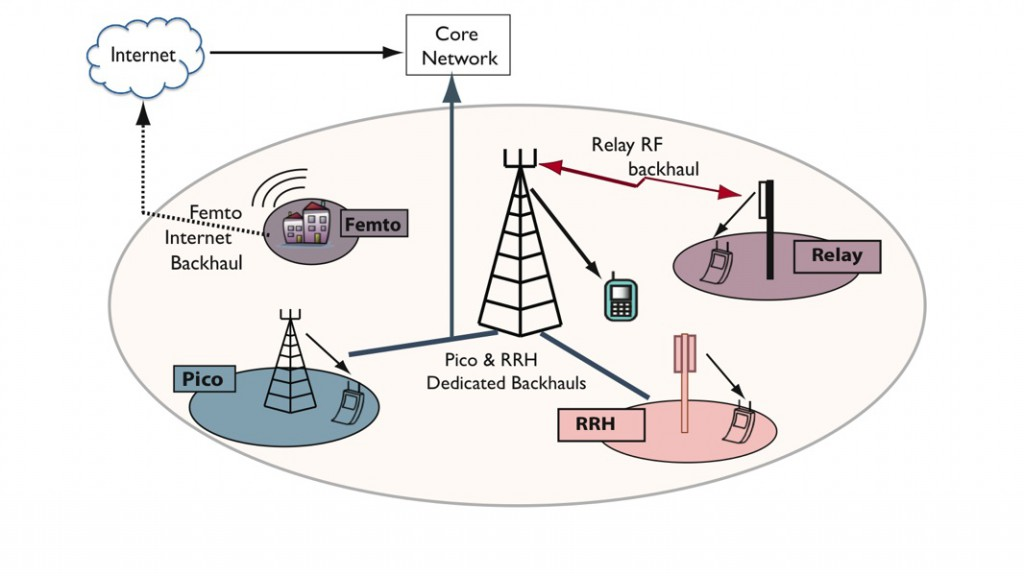
\includegraphics[scale=.2]{het_net}
\end{frame}


\section{General Setup}

\begin{frame}

\frametitle{General Problem Formulation}
\begin{enumerate}
\setlength\itemsep{2em}

\item  Player $f$ has beamforming matrix $\mathbf{U}_f$ as strategy
\begin{itemize}
\item $\mathbf{U}_f$ has an implied power allocation
\end{itemize}
%\item Simplify by selecting $\mathbf{U}_f$ as a pseudo inverse of $\mathbf{H}_f$  (i.e $\mathbf{H}_f\mathbf{U}_f = \mathbf{I}$) such that 
%	\begin{equation*}
%	\gamma_{f,i} = \frac{\|\mathbf{h}^H_{f,i}\mathbf{u}_{f,i}\|^2}
%	{\sigma^2_{\text{noise}}}
%	\end{equation*}
%	with 
%	\begin{equation*}
%	U_{f}(\boldsymbol{\gamma}_{f}) =
%	\sum_{i=1}^{K_{f}}
%    	 U_{f,i}(\gamma_{f,i}) .
%	\end{equation*}
\pause
Does the problem admit the N-Person Concave game Framework? 

\item  Set of strategies is convex \faThumbsOUp
\pause
\item  $U_{f}(\boldsymbol{\gamma}_{f})$ is concave only when $U_{f,i}(\gamma_{f,i})$ is concave and non-increasing 
\faThumbsODown
\end{enumerate}
\end{frame}

\section{Convex Setup}

\begin{frame}
\frametitle{Convex Problem Formulation}
\begin{enumerate}
\setlength\itemsep{2em}
\item Pre-select $\mathbf{U}_f$ to be a psuedo inverse of $\mathbf{H}_f$  (i.e $\mathbf{H}_\mathrm{f}\mathbf{U}_\mathrm{f} = \mathbf{I}$).
\item 
	Normalize the columns of $\mathbf{U}_{f}$ such that 
	 $\|\mathbf{u}_{f,i}\|^2 =1 \;\forall i \in \{1 ... K_{f}\}$.
\item 
	Player $f$ strategy is now the diagonal, power allocation  	
	matrix $\mathrm{diag}(\mathbf{p}_{f})$ with $p_{f,i} \geq 0, \forall i \in \{1 ... K_{f}\}$
such that the transmitted 		
	signal is 
	$\mathbf{s}_{f	}= \mathbf{U}_{f} 
	\mathrm{diag}(\mathbf{p}_{f})^{\frac{1}{2}}
	\mathbf{x}_{f}$.
\item 
	Power constraint given by 
	\begin{gather*}
	\sum_{i=1}^{K_{f}} p_{f,i}
	  \leq P^{Total}_{f}.
	  	\end{gather*}
\end{enumerate}
\end{frame}

\begin{frame}
\frametitle{Problem Analysis}
Does the problem admit the N-Person Concave game Framework? 
\\
\begin{enumerate}
\setlength\itemsep{2em}
\item  Set of strategies is convex \faThumbsOUp
\item  $U_{f}(\boldsymbol{\gamma}_{f})$ is concave if 
	$U_{f,i}(\cdot)$ is non-decreasing and concave (reasonable assumption) \faThumbsOUp
\item 
	If $U_{f,i}(\cdot)$ is strictly concave, this satisfies conditions for the unique Normalized Nash Equilibrium (Diagonally Strict Concavity)  \faThumbsOUp
\end{enumerate}

\end{frame}



\section{A Solution}
\begin{frame}
\frametitle{Player Optimization Problem}
Each player attempts to solve the optimization problem given by 
	\begin{subequations}
	\begin{align}
	    \underset{\mathbf{p}_{f} }{\text{min}} \;
	    & - \sum_{i=1}^{K_f}
    	U_{f,i}(\gamma_{f,i}) \label{player_opt_c} \\
	    \text{subject to  }\\
	  &
	  \sum^F_{f=1} E\{ \mathbf{\tilde{h}}_{m,f}^T  \mathbf{s}_{f} 						
	\mathbf{s}_{f}^{H} \mathbf{\tilde{h}}_{m,f}^* \}
	\leq I^{Threshold}		
	_{m} & m \in \{1 ...m\} 
		\label{interference_const_c}\\
        & 
        	\sum_{i=1}^{K_{f}} p_{f,i}
	   \leq P_{f}^{\text{Total}}  \label{power_const_c}\\
        & p_{f,i} \geq 0 &  i\in \{1 ...K_{f}\} \label{pos_power_const_c}
	\end{align}
	\end{subequations}

Note that $\mathbf{U}_{f}$ is pre-selected as a pseudo-inverse to  $\mathbf{H}_f$.
\end{frame}


\begin{frame}
\frametitle{Steps Outline}
\begin{enumerate}
\setlength\itemsep{2em}

\item
	Form Potential Function.
\item
	Setup distributed algorithm.
\end{enumerate}
\end{frame}

\begin{frame}
\frametitle{The Potential Function}
Things to note
\begin{enumerate}
\item
	Spacing assumption makes $U_{f}(\boldsymbol{\gamma}_{f})$ independent of all other player strategies. 

\item
	The sum of concave functions over a convex set is also concave. Does this satisfy the potential function condition?
	\begin{equation*}\label{potential_game_condition}
\frac{\partial \Psi(\boldsymbol{\gamma})}{\partial \boldsymbol{\gamma}_{f}}
 =
 \frac{\partial U_f(\boldsymbol{\gamma})}{\partial \boldsymbol{\gamma}_{f}}
\end{equation*} 
Yes!
\end{enumerate}

\end{frame}

\begin{frame}
\frametitle{Solving for a NNE}
\begin{enumerate}
\setlength\itemsep{2em}

\item
	The potential function of a game with strictly concave utility functions has optimum corresponding to NNE.
\item
	Satisfying the Diagonally Strict Concavity conditions means the NNE is unique.
\end{enumerate}
\bigskip
Just need to solve for the unique optimum of a convex problem.
\pause
\par
 Can the problem be distributed?
\end{frame}

\begin{frame}
\frametitle{Distributed Dual Ascent}
For $U_{f,i}(\gamma_{f,i}) = log(1+\gamma_{f,i})$ and potential function
\begin{gather*} \label{Potential_Function}
\Psi(\mathbf{p}) = \sum_{f = 1}^{F} U_{f}(\mathbf{p}_{f}).
\end{gather*}
We arrive at a central, convex optimization problem given by
		\begin{subequations}
	\label{optim}
	\begin{align}
	    \underset{\mathbf{p}}{\text{minimize  }}
	    & \; \Psi(\mathbf{p}) \label{potential_game} \\
	    \text{subject to  } \; &
	  \sum^F_{f=1} E\{\tilde{\mathbf{h}}_{m,f}^T  \mathbf{s}_{f} 						
	\mathbf{s}_{f}^{H} \tilde{\mathbf{h}}_{m,f}^* \}\leq I^{Threshold}		
	_{m} & m \in \{1 ...m\} 
		\label{interference_const}\\
        & E\{trace(\mathbf{s}_f\mathbf{s}_f^H)\}  \leq P_{f}^{\text{Total}}  \label{power_const}
        & \forall f \in \{1 ... f\}\\
        & p_{f,i} \geq 0 &  \forall i \in \{1 ...K_{f}\} \; \forall f \in \{1 ... F\}\label{pos_power_const}
	\end{align}
	\end{subequations}.
\end{frame}


\section{Simulation Results}

\begin{frame}
\frametitle{Expected Results}
\begin{enumerate}
\setlength\itemsep{2em}

\item
	When players have sufficient power, at least one interference constraint should be active.
\item
	With sufficient power, increasing the number of antennas at the base stations should allow for higher utility.
\item
	The choice of the psuedoinverse, $\mathbf{U}_{f}$, should be further optimized. 
\end{enumerate}
\end{frame}


\begin{frame}
\frametitle{Multiple Antennas with Constant Power}
\begin{figure}
	\includegraphics[width=\textwidth]{results/central_antenna}
	\caption{With $K_f = 5$ (users) and $T_f = 15$ (antennas), increasing antennas allows players with constant power to increase utility.}
\end{figure}
\end{frame}

\begin{frame}
\frametitle{Increasing Power at FCBS}
\begin{figure}
	\includegraphics[width=\textwidth]{results/central_power}
	\caption{For $K_f = 5$ and $T_f = 15$, increasing FCBS power constraint is limited by interference.}
\end{figure}
\end{frame}

\begin{frame}
\frametitle{Selecting the Beamformer}
\begin{figure}
	\includegraphics[width=\textwidth]{results/central_beamformer}
\caption{With $K_f = 5$ (users) and $T_f = 10$ (antennas), choice of $\mathbf{U}_{f}$ may depend on the active system constraints.}
\end{figure}
\end{frame}

\section{Conclusion}
\begin{frame}
\frametitle{Continuing Work}
\begin{enumerate}
\item
	Implement distributed version.
\item
	Improve choice of beamformer using additional DOF. 
\item
	Consider "fairness" with respect to FCBS utility.
\end{enumerate}
\end{frame}

\begin{frame}
  \centering \Large
  \emph{Thank You.}
  \\
	\bigskip
    \centering \Large
  \emph{Questions or Comments?}
\end{frame}

\end{document}
